\documentclass[10pt]{article}
\usepackage{acronym}
\usepackage{amsfonts}
\usepackage{amsmath}
\usepackage{graphicx}
\usepackage{amsthm}
\usepackage{Steven}
\usepackage{subfigure}

%\newtheorem{proposition}{Proposition}
\DeclareMathOperator{\var}{Var}
\DeclareMathOperator{\cov}{Cov}

\oddsidemargin -0.5in
\evensidemargin -0.5in
\textwidth 7.5in
\topmargin -0.5in
\textheight 9in

\title{Research Results}

\begin{document}
\maketitle
\tableofcontents
\listoffigures
\section*{Acronyms Used In This Document}
\begin{acronym}
	\acro{MC}{Monte Carlo}
	\acro{AV}{antithetic variables}
	\acro{PAV}{parameterized antithetic variables}
	\acro{CRLB}{Cramer Rao Lower Bound}
	\acro{PDF}{probability density function}
	\acro{MVU}{minimum variance unbiased}
\end{acronym}

\section{Single Link}

We consider the case where a single source is transmitting a sequence of packets to a single destination (Figure~\ref{fig:single_link}) and the source records the outcome ($X_{1}^{(n)}$ of the packet. Examples of outcomes are loss information or delay information; we consider loss based tomography. In this case, the outomes are Bernoulli random variables, with $X_{1}^{(n)}=1$ with probability $\alpha$ denoting successful reception of the packet. We are interested in developing an unbiased estimator for the link success probability $\alpha$ with a low variance.

\begin{figure}[ht!]
\centering
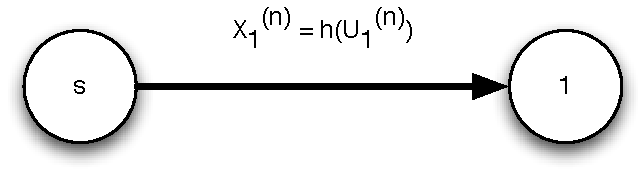
\includegraphics[width=0.4\columnwidth]{img/single_link}
\caption{Single Link}\label{fig:single_link}
\end{figure}
\subsection{Loss Base Tomography}
\subsubsection{Monte Carlo Estimation}
The simplest estimation technique is \ac{MC}. We generate a sequence of unifrom random variables $U_{1}^{(n)}$ and transforming them to Bernoulli random variables $X_{1}^{(n)} = h(U_{1}^{(n)}) = \mathbb{I}_{U_{1}^{(n)} < \alpha}$. The \ac{MC} estimator is then

\begin{equation}
\hat{\alpha}_{MC} = \frac{1}{n}\displaystyle\sum_{i=1}^{n}X_{1}^{(i)}
\end{equation}

This is clearly unbiased and has a normalized variance of

\begin{equation}
n\var\left(\hat{\alpha}_{MC}\right) = \alpha(1-\alpha)
\end{equation}

The variance as a function of $\alpha$ is shown in Figure~\ref{fig:mc}. The variance (or mean squared error since the estimator is ubiased) is maximum at $\alpha = \frac{1}{2}$.
\begin{figure}[ht!]
\centering
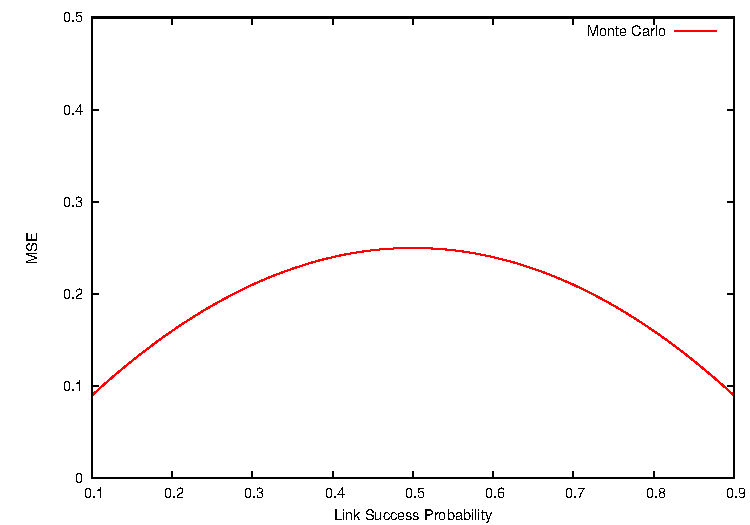
\includegraphics[width=0.5\columnwidth]{img/monte_carlo}
\caption[Normalized variance for \acs{MC} as a function of link success probability, $\alpha$]{Normalized variance for \acf{MC} as a function of link success probability, $\alpha$}\label{fig:mc}
\end{figure}

\subsubsection{Antithetic Variables}
Our first step towards improving over the simple \ac{MC} estimation is the use of \ac{AV}\cite{ross-2006}. The idea here is that instead of generating a sequence with $n$ random variables, we generate a sequence of length $\frac{n}{2}$ and form the estimator

\begin{equation}
\hat{\alpha}_{AV} = \frac{1}{n}\displaystyle\sum_{i=1}^{n/2}h(U_{1}^{(i)})+h(1 - U_{1}^{(i)})\label{eq:av}
\end{equation}

Because expectation is linear and because $h(U_{1}^{(n)})$ and $h(1-U_{1}^{(i)})$ are identically distributed, it is easy enough to verify that the estimator is unbiased. The normalized variance is given as

\begin{align*}
n\var\left(\hat{\alpha}_{AV}\right) &= \frac{1}{n}\sum_{i=1}^{n/2}\var\left(h(U_{1}^{(i)}) + h(1-U_{1}^{(i)})\right)\\
&=\frac{\var\left(h(U_{1}^{(i)})\right) + \var\left(h(1-U_{1}^{(i)})\right) + 2\cov\left(h(U_{1}^{(i)}),h(1-U_{1}^{(i)})\right)}{2}\\
&=\var\left(h(U_{1}^{(i)})\right) + \cov\left(h(U_{1}^{(i)}),h(1-U_{1}^{(i)})\right)\\
&=\mathbb{E}\left[h(U_{1}^{(i)})^2\right] + \mathbb{E}\left[h(U_{1}^{(i)})h(1-U_{1}^{(i)})\right] - 2\mathbb{E}\left[h(U_{1}^{(i)})\right]^{2}
\end{align*}

\begin{equation}
n\var\left(\hat{\alpha}_{AV}\right)=\alpha+ 2\mathbb{I}_{\alpha > \frac{1}{2}}(\alpha-\frac{1}{2})-2\alpha^{2}\label{eq:av_var}
\end{equation}

\begin{figure}[ht!]
\centering
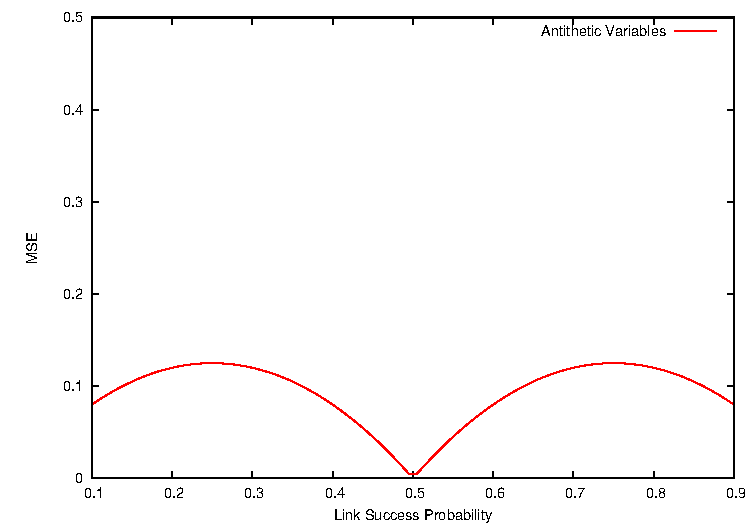
\includegraphics[width=0.5\columnwidth]{img/av}
\caption[Normalized variance for \acs{AV} as a function of link success probability, $\alpha$]{Normalized variance for \acf{AV} as a function of link success probability, $\alpha$}\label{fig:av}
\end{figure}

The normalized variance as a function of $\alpha$ is shown in Figure~\ref{fig:av}. Note that the normalized variance is maximum at $\alpha = \frac{1}{4}$ and $\alpha = \frac{3}{4}$. From this figure we observe:
\begin{proposition}\label{prop:av}
\[
\var\left(\hat{\alpha}_{AV}\right) < \var\left(\hat{\alpha}_{MC}\right), \forall \alpha \in (0,1)
\]
\end{proposition}

\begin{proof}
First, consider when $\alpha < \frac{1}{2}$
\[
\alpha - 2\alpha^2  <  \alpha(1-\alpha)
\]
\[
\alpha - 2\alpha^2  <  \alpha-\alpha^2
\]
\[
0  <  \alpha^2
\]
Next consider when $\alpha > \frac{1}{2}$
\[
3\alpha - 1 - 2\alpha^2 < \alpha - \alpha^{2}
\]
\[
0 < \alpha^2 - 2\alpha + 1
\]
\[
0 < (\alpha - 1)^2
\]
Finally, when $\alpha = \frac{1}{2}$ we have $\var\left(\hat{\alpha}_{AV}\right) = 0$ and $\var\left(\hat{\alpha}_{MC}\right) = \frac{1}{4}$
\end{proof}
Using \ac{AV}, we have the greatest variance reduction when the variance of the \ac{MC} estimator is at its maximum. The closer $\alpha$ is to either $0$ or $1$, there is less variance reduction.

\subsubsection{Parameterized Antithetic Variables}
We wish to develop an estimator with a tunable parameter $\beta$ such that the variance reduction is maximized when $\beta=\alpha$, but which is an unbiased estimator for all $\alpha$ and all $\beta$.

Consider $\alpha$ fixed and unknown and to be estimated, and $\beta \in [0,1]$ chosen based on some prior assumptions about $\alpha$. Generate $U_{1}^{(n)} \sim \mathrm{Uni}(0,\beta)$ and from there set
\begin{equation}
\bar{U}_{1}^{(n)} = \frac{1-\beta}{\beta} U_1 + \beta.
\end{equation}
Note that $\bar{U}_{1}^{(n)} \sim \mathrm{Uni}(\beta,1)$. We consider an estimator of the form
\begin{equation}
\hat{\alpha}_{PAV} = \frac{1}{n} \sum_{i=1}^{n/2} \left( \beta \left( \mathbf{1}_{U_{1}^{(i)} \leq \alpha} + \mathbf{1}_{\beta-U_{1}^{(i)} \leq \alpha} \right) + (1-\beta) \left( \mathbf{1}_{\bar{U}_{1}^{(i)} \leq \alpha} + \mathbf{1}_{1-\bar{U}_{1}^{(i)} + \beta < \alpha} \right) \right)
\end{equation}
Then it is straightforward to show
\begin{eqnarray}
\Ebb[\hat{\alpha}_{PAV}] &=& \frac{1}{2} \left[ \beta \left( \Pbb(U_1 \leq \alpha) + 1 - \Pbb(U_1 \leq \beta - \alpha) \right) + (1-\beta) \left( \Pbb(\bar{U}_1 \leq \alpha) + 1 - \Pbb( \bar{U}_1 \leq 1+ \beta - \alpha) \right) \right] \nonumber \\
&=& \left\{ \begin{array}{ll}
\frac{1}{2} \left[ \beta \left( \frac{\alpha}{\beta} + 1 - \frac{\beta-\alpha}{\beta} \right) + (1-\beta) \left(0 + 1 - 1 \right) \right] , \; & \alpha \leq \beta \\
\frac{1}{2} \left[ \beta \left(1 + 1 - 0 \right) + (1-\beta) \left( \frac{\alpha-\beta}{1-\beta} + 1 - \frac{1+\beta-\alpha-\beta}{1-\beta} \right) \right], \; & \alpha > \beta 
\end{array} \right. \nonumber \\
&=& \alpha
\end{eqnarray}

We can then find the normalized variance as
\begin{equation}n\var(\hat{\alpha}_{PAV}) = \left\{
\begin{array}{llll}
(\alpha-\beta)(\beta-(2\alpha-1)), & \alpha \leq \frac{1}{2} & \beta \leq \alpha & \\
(\beta-\alpha)(2\alpha-\beta), & & \alpha < \beta \leq 2 \alpha &  \\
\alpha(\beta-2\alpha), & & \beta > 2 \alpha & \\
(1-\alpha)((2\alpha-1)-\beta), & \alpha > \frac{1}{2} & \beta \leq \alpha & \beta \leq 2 \alpha - 1 \\
(\alpha-\beta)(\beta - (2\alpha-1)), & & \beta \leq \alpha & 2 \alpha - 1 < \beta \\
(\beta-\alpha)(2\alpha-\beta), & & \beta > \alpha 
\end{array}\right.
\end{equation}

The normalized variance for both \ac{AV} and \ac{PAV} is shown in Figure~\ref{fig:pav}.
\begin{figure}[ht!]
\centering
\subfigure[$\alpha = 0.2$]{
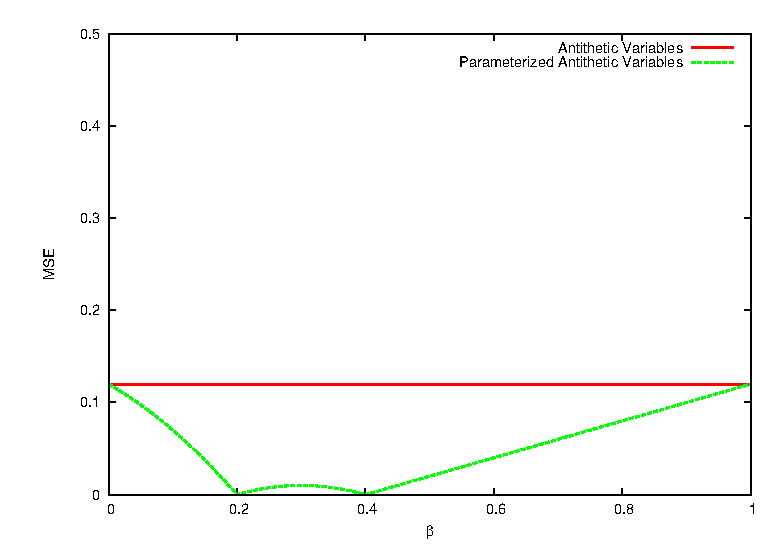
\includegraphics[width=0.4\columnwidth]{img/pav_2}
\label{fig:subfig1}
}
\subfigure[$\alpha = 0.4$]{
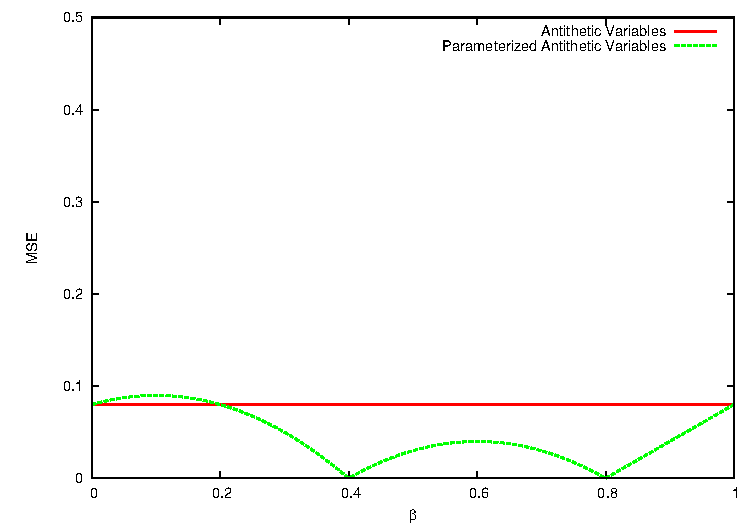
\includegraphics[width=0.4\columnwidth]{img/pav_4}
\label{fig:subfig2}
}
\subfigure[$\alpha = 0.6$]{
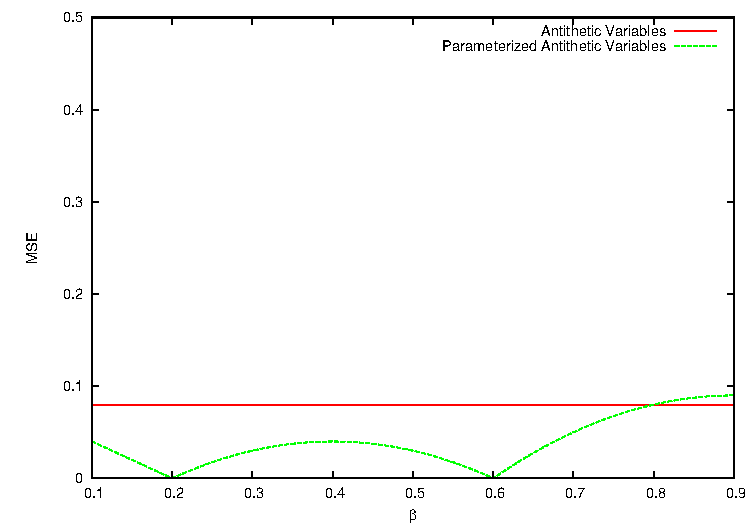
\includegraphics[width=0.4\columnwidth]{img/pav_6}
\label{fig:subfig3}
}
\subfigure[$\alpha = 0.8$]{
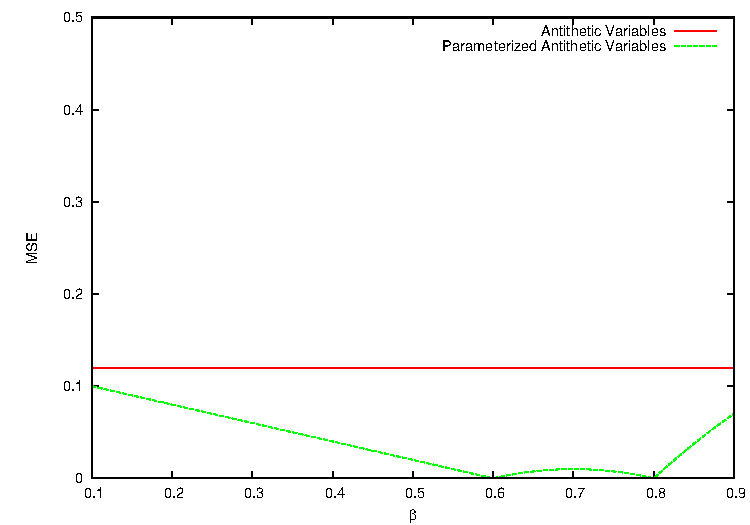
\includegraphics[width=0.4\columnwidth]{img/pav_8}
\label{fig:subfig4}
}
\label{fig:subfigureExample}
\caption[Normalized variance for \acs{PAV}]{Normalized variance for \acf{PAV}: \subref{fig:subfig1} $\alpha = 0.2$, \subref{fig:subfig2} $\alpha = 0.4$, \subref{fig:subfig3} $\alpha = 0.6$, and \subref{fig:subfig4} $\alpha = 0.8$}\label{fig:pav}
\end{figure}

\begin{proposition}\label{prop:pav}
\[
\var\left(\hat{\alpha}_{PAV}\right) < \var\left(\hat{\alpha}_{MC}\right), \forall \alpha,\beta \in (0,1)
\]
\end{proposition}
\begin{proof}
If $\alpha < \frac{1}{3}$, then $\displaystyle\max_{\beta}\var\left(\hat{\alpha}_{PAV}\right)=\alpha-2\alpha^2$; we are doing no worse than \ac{AV}. We proved in Proposition~\ref{prop:av} that \ac{AV} is always better than \ac{MC}. If $\frac{1}{3} < \alpha < \frac{1}{2}$, then $\displaystyle\max_{\beta}\var\left(\hat{\alpha}_{PAV}\right)=\frac{(1-\alpha)^2}{4}$.
\[
\frac{(1-\alpha)^2}{4} < \alpha(1-\alpha)
\]
\[
\frac{(1-\alpha)}{4} < \alpha
\]
\[
1-\alpha < 4\alpha < 4\frac{1}{2}
\]
\[
1-\alpha < 2
\]
Because $\alpha\in[0,1]$, the above is true and we conclude that $\var\left(\hat{\alpha}_{PAV}\right) < \var\left(\hat{\alpha}_{AV}\right)$ for $\alpha < \frac{1}{2}$.

If $\alpha > \frac{2}{3}$, then  $\displaystyle\max_{\beta}\var\left(\hat{\alpha}_{PAV}\right)=\alpha+2(\alpha-\frac{1}{2})-2\alpha^2$; again we are doing no worse than \ac{AV}. If $\frac{1}{3} < \alpha < \frac{1}{2}$, then $\displaystyle\max_{\beta}\var\left(\hat{\alpha}_{PAV}\right)=\frac{\alpha^2}{4}$.
\[
\frac{\alpha^2}{4} < \alpha(1-\alpha)
\]
\[
\frac{\alpha}{4} < 1-\alpha
\]
\[
\alpha < 4(1-\alpha) < 4\frac{1}{2}
\]
\[
\alpha < 2
\]
Because $\alpha\in[0,1]$, the above is true and we conclude that $\var\left(\hat{\alpha}_{PAV}\right) < \var\left(\hat{\alpha}_{AV}\right)$ for $\alpha > \frac{1}{2}$.

\end{proof}
\begin{corollary}
If $\alpha < \frac{1}{3}$ or $\alpha > \frac{2}{3}$, then
\[
\var\left(\hat{\alpha}_{PAV}\right) < \var\left(\hat{\alpha}_{AV}\right), \forall \beta \in (0,1)
\]
\end{corollary}

\begin{corollary}
If $\beta \geq 3\alpha -1,~\alpha \in (\frac{1}{3},\frac{1}{2})$ or $\beta \leq 3\alpha -1,~\alpha \in (\frac{1}{2},\frac{2}{3})$, then
\[
\var\left(\hat{\alpha}_{PAV}\right) < \var\left(\hat{\alpha}_{AV}\right)
\]
\end{corollary}

\begin{corollary}
If $\alpha \in (\frac{1}{3},\frac{1}{2})$ and $\beta < 3\alpha -1$, then the worst case choice of $\beta$ is
\[
\frac{3\alpha - 1}{2}
\]
which gives
\[
\var\left(\hat{\alpha}_{PAV}\right) =\left(\frac{1-\alpha}{2}\right)^2
\]
If $\alpha \in (\frac{1}{2},\frac{2}{3})$ and $\beta > 3\alpha -1$, then the worst case choice of $\beta$ is
\[
\frac{3\alpha}{2}
\]
which gives
\[
\var\left(\hat{\alpha}_{PAV}\right) =\left(\frac{\alpha}{2}\right)^2
\]
\end{corollary}

The ratio of \ac{PAV} variance to \ac{AV} variance is plotted in Figure~\ref{fig:ratio}.

\begin{figure}
\centering
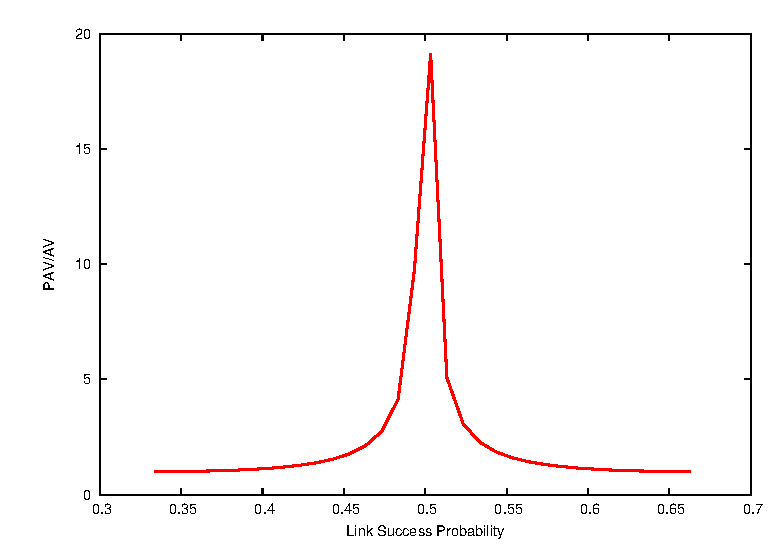
\includegraphics[width=0.5\columnwidth]{img/ratio}
\caption[Ratio of \acs{PAV} to \acs{AV} as a function of link success probability, $\alpha$]{Ratio of \acf{PAV} to \acf{AV} as a function of link success probability, $\alpha$}\label{fig:ratio}
\end{figure}

\subsubsection{Cramer Rao Lower Bounds}
\paragraph{Monte Carlo}
If we let $m = \displaystyle\sum_{i=1}^nX_1^{(i)}$ denote the number of successful packet receptions, we can then write
\begin{equation}
p(\xbf;\alpha)=\displaystyle\prod_{i=1}^{m}\alpha\prod_{i=m+1}^{n}(1-\alpha)\label{eq:pdf}
\end{equation}
We first check to make sure the assumed \ac{PDF} meets the condition that
\begin{equation}
\Ebb\left[\frac{\partial \ln p(\xbf;\alpha)}{\partial\alpha}\right]=0,~\forall \alpha
\end{equation}

This is known as the ``regularity'' condition.
\[
\Ebb\left[\frac{\partial \left(m\ln\alpha + (m-n)\ln(1-\alpha)\right)}{\partial\alpha}\right]=\Ebb\left[\frac{m}{\alpha}+\frac{(m-n)}{1-\alpha}\right]
\]
\[
\frac{1}{\alpha}\Ebb\left[m\right]+\frac{1}{1-\alpha}\Ebb\left[m\right]-\frac{N}{1-\alpha}
\]
\[
\frac{\Ebb[m]}{\alpha(1-\alpha)}-\frac{N}{1-\alpha}=\frac{N}{1-\alpha}-\frac{N}{1-\alpha}
\]
The assumed \ac{PDF} meets the regularity condition and therefore the variance of any unbiased estimator $\hat{\alpha}$ must satisfy
\begin{equation}
\var\left(\hat{\alpha}\right) \geq \frac{1}{-\Ebb\left[\frac{\partial^2\ln p(\xbf;\alpha)}{\partial\alpha^2}\right]}
\end{equation}

\[
\Ebb\left[\frac{\partial^2\ln p(\xbf;\alpha)}{\partial\alpha^2}\right] = \Ebb\left[-\frac{m}{\alpha^2} + \frac{(m-n)}{(1-\alpha)^2}\right]
\]
\[
-\frac{n}{\alpha}+\frac{n\alpha}{(1-\alpha)^2)}-\frac{n}{(1-\alpha)^2)}=-\frac{n}{\alpha(1-\alpha)}
\]
\begin{equation}
\var\left(\hat{\alpha}\right) \geq \frac{\alpha(1-\alpha)}{n}\label{eq:crlb}
\end{equation}
Because the sample average attains this variance, we know that it is a \ac{MVU} estimator for $\alpha$. Although this result my seem inconsistent with our results above for \ac{AV} and \ac{PAV}, it is not. The reason is that an estimator can have variance no lower than (\ref{eq:crlb}) for the assumed \ac{PDF} in (\ref{eq:pdf}) - the assumed \ac{PDF} is different for the \ac{AV} and \ac{PAV} and hence the variance for an unbiased estimator may be lower.

\paragraph{Antithetic Variables}
If we let
\[ Z_i = \frac{h(U_{1}^{(i)})+h(1 - U_{1}^{(i)})}{2}\]
then we can rewrite (\ref{eq:av}) as
\begin{equation*}
\hat{\alpha}_{AV} = \frac{2}{n}\displaystyle\sum_{i=1}^{n/2}Z_i
\end{equation*}
The \ac{PDF} for $Z_i$ is
\begin{equation}
\Pbb[Z_i = z] = \left\{
\begin{array}{lr}
(1-2\alpha)^{+} & z = 0\\
2\min(\alpha, 1-\alpha) & z = \frac{1}{2}\\
(2\alpha - 1)^{+} & z = 1
\end{array}\right.
\end{equation}
We can now calculate the \ac{CRLB} for the antithetic variable case. If $\alpha < \frac{1}{2}$ and we let $m$ be the number of $Z_i=0$, then
\[p(\zbf;\alpha) = (1-2\alpha)^m(2\alpha)^{(\frac{n}{2}-m)}\]
\[\ln p(\zbf;\alpha) = m\ln(1-2\alpha) + (\frac{n}{2}-m)\ln(2\alpha)\]
\[\frac{\partial \ln p(\xbf;\alpha)}{\partial\alpha} = \frac{-2m}{1-2\alpha} + (\frac{n}{2}-m)\frac{1}{\alpha}\]
\[\Ebb\left[\frac{\partial \ln p(\xbf;\alpha)}{\partial\alpha}\right] = \frac{-2\Ebb[m]}{1-2\alpha} + (\frac{n}{2}-\Ebb[m])\frac{1}{\alpha}\]
\[\Ebb[m] = (1-2\alpha)\frac{n}{2}\]
\[\Ebb\left[\frac{\partial \ln p(\xbf;\alpha)}{\partial\alpha}\right] = 0 \]
The \ac{PDF} meets the regularity conditions.
\[\frac{\partial^2 \ln p(\xbf;\alpha)}{\partial\alpha^2} = \frac{-4m}{(1-2\alpha)^2} + (\frac{n}{2}-m)\frac{-4}{(2\alpha)^2}\]
\[\Ebb\left[\frac{\partial^2 \ln p(\xbf;\alpha)}{\partial\alpha^2}\right] = \frac{-2n}{(1-2\alpha)(2\alpha)}\]
The \ac{CRLB} then is
\begin{equation}
n\var\left(\hat{\alpha}_{AV}\right) \geq \alpha -2\alpha^2\label{eq:av_crlb}
\end{equation}
Comparing (\ref{eq:av_crlb}) with (\ref{eq:av_var}) we see that the \ac{CRLB} is attained. It can be shown in a similar manner that the bound is achieved when $\alpha > \frac{1}{2}$. Therefore (\ref{eq:av}) is efficient.

\paragraph{Parameterized Anithetic Variables}
\begin{quote}
I need to find the assumed \ac{PDF} for \ac{PAV} before I can calculate the \ac{CRLB}.
\end{quote}

\subsection{Delay Based Tomography}

\section{Two Links}
We extend the previous analysis as before but now for the two link case.
\subsection{Monte Carlo Estimation}
We generate two sequences of unifrom random variables $U_{1}^{(n)}$ and $U_{2}^{(n)}$ and transforming them to Bernoulli random variables $X_{i}^{(n)} = h(U_{i}^{(n)}) = \mathbb{I}_{U_{i}^{(n)} < \alpha_i}$. The Monte Carlo estimator is then

\begin{equation}
\hat{\alpha}_{MC} = \frac{1}{n}\displaystyle\sum_{i=1}^{n}X_{1}^{(i)}X_{2}^{(i)}
\end{equation}

This is clearly unbiased and has a normalized variance of

\begin{equation}
n\var\left(\hat{\alpha}_{MC}\right) = \alpha_1\alpha_2(1-\alpha_1\alpha_2)
\end{equation}

\subsection{Antithetic Variables}
The antithetic variable estimator is now

\begin{equation}
\hat{\alpha}_{AV} = \frac{1}{n}\displaystyle\sum_{i=1}^{n/2}h(U_{1}^{(i)})h(U_{2}^{(i)})+h(1 - U_{1}^{(i)})h(1 - U_{2}^{(i)})
\end{equation}

As before, because expectation is linear and because $h(U_{i}^{(n)})$ and $h(1-U_{i}^{(n)})$ are identically distributed, it is easy enough to verify that the estimator is unbiased. For ease of notation, we replace $h(U_{i}^{(i)})h(U_{2}^{(i)})$ with $g(\Ubf^{(i)})$. The normalized variance is given as

\begin{align*}
n\var\left(\hat{\alpha}_{AV}\right) &= \frac{1}{n}\sum_{i=1}^{n/2}\var\left(g(\Ubf^{(i)}) + g(1-\Ubf^{(i)})\right)\\
&=\frac{\var\left(g(\Ubf^{(i)})\right) + \var\left(g(1-\Ubf^{(i)})\right) + 2\cov\left(g(\Ubf^{(i)}),g(1-\Ubf^{(i)})\right)}{2}\\
&=\var\left(g(\Ubf^{(i)})\right) + \cov\left(g(\Ubf^{(i)}),g(1-\Ubf^{(i)})\right)\\
&=\mathbb{E}\left[g(\Ubf^{(i)})^2\right] + \mathbb{E}\left[g(\Ubf^{(i)})g(1-\Ubf^{(i)})\right] - 2\mathbb{E}\left[g(\Ubf^{(i)})\right]^{2}\\
&=\alpha_1\alpha_2+ 4\mathbb{I}_{\alpha_1 > \frac{1}{2},\alpha_2 > \frac{1}{2}}(\alpha_1-\frac{1}{2})(\alpha_2 > \frac{1}{2})-2\alpha_1^{2}\alpha_2^2
\end{align*}

\subsection{Parameterized Antithetic Variables}
When we extend the proposed technique of parameterized antithetic variables, we obtain the following estimator
\begin{align}
\hat{\alpha}_{PAV} & = & \frac{1}{n} \sum_{i=1}^{n/2} \beta \left( \mathbf{1}_{U_{1}^{(i)} \leq \alpha_1,U_{2}^{(i)} \leq \alpha_2} + \mathbf{1}_{\beta-U_{1}^{(i)} \leq \alpha_1,\beta-U_{2}^{(i)} \leq \alpha_2} \right) +\\
&  & (1-\beta) \left( \mathbf{1}_{\bar{U}_{1}^{(i)} \leq \alpha_1,\bar{U}_{2}^{(i)} \leq \alpha_2} + \mathbf{1}_{1-\bar{U}_{1}^{(i)} + \beta < \alpha_1,1-\bar{U}_{2}^{(i)} + \beta < \alpha_2} \right)
\end{align}
Unfortunately, this is a biased estimator. The bias for this particular estimator is dependent upon both the choice of $\beta$ and $\alpha$ and so it can not be adjusted for.

\nocite{*}
\bibliographystyle{plain}
\bibliography{sources}
\end{document}